%  ========================================================================
%  Copyright (c) 1985-2014 The University of Washington
%
%  Licensed under the Apache License, Version 2.0 (the "License");
%  you may not use this file except in compliance with the License.
%  You may obtain a copy of the License at
%
%      http://www.apache.org/licenses/LICENSE-2.0
%
%  Unless required by applicable law or agreed to in writing, software
%  distributed under the License is distributed on an "AS IS" BASIS,
%  WITHOUT WARRANTIES OR CONDITIONS OF ANY KIND, either express or implied.
%  See the License for the specific language governing permissions and
%  limitations under the License.
%  ========================================================================
%

% Documentation for University of Washington thesis LaTeX document class
% by Jim Fox
% fox@washington.edu
%
%    Revised for version 2015/03/03 of uwthesis.cls
%
%    This document is contained in a single file ONLY because
%    I wanted to be able to distribute it easily.  A real thesis ought
%    to be contained on many files (e.g., one for each chapter, at least).
%
%    To help you identify the files and sections in this large file
%    I use the string '==========' to identify new files.
%
%    To help you ignore the unusual things I do with this sample document
%    I try to use the notation
%       
%    % --- sample stuff only -----
%    special stuff for my document, but you don't need it in your thesis
%    % --- end-of-sample-stuff ---


%    Printed in twoside style now that that's allowed
%
 
\documentclass [11pt, proquest] {uwthesis}[2015/03/03]
 
%
% The following line would print the thesis in a postscript font 

% \usepackage{natbib}
% \def\bibpreamble{\protect\addcontentsline{toc}{chapter}{Bibliography}}

\setcounter{tocdepth}{1}  % Print the chapter and sections to the toc
 

% ==========   Local defs and mods
%

% --- sample stuff only -----
% These format the sample code in this document

\usepackage{alltt}  % 
\newenvironment{demo}
  {\begin{alltt}\leftskip3em
     \def\\{\ttfamily\char`\\}%
     \def\{{\ttfamily\char`\{}%
     \def\}{\ttfamily\char`\}}}
  {\end{alltt}}
 
% metafont font.  If logo not available, use the second form
%
% \font\mffont=logosl10 scaled\magstep1
\let\mffont=\sf
% --- end-of-sample-stuff ---
 
\usepackage{graphicx}
\graphicspath{ {figures/} }


\begin{document}
 
% ==========   Preliminary pages
%
% ( revised 2012 for electronic submission )
%

\prelimpages
 
%
% ----- copyright and title pages
%
\Title{Smart Things and Cochlear Implants}
\Author{Tyler Ganter}
\Year{1985-2014}
\Program{UW Information Technology}

\Chair{Name of Chairperson}{Title of Chair}{Department of Chair}
\Signature{First committee member}
\Signature{Next committee member}
\Signature{etc}

% \copyrightpage

% \titlepage  

% --- sample stuff only -----
% unusual footnote not found in a real thesis
% You just use the \titlepage as commented out above

{\Degreetext{A dissertation%
  \footnote[2]{an egocentric imitation, actually}\\
  submitted in partial fulfillment of the\\ requirements for the degree of}
 \def\thefootnote{\fnsymbol{footnote}}
 \let\footnoterule\relax
 \titlepage
 }
\setcounter{footnote}{0}

% --- end-of-sample-stuff ---
 
%
% ----- signature and quoteslip are gone
%

%
% ----- abstract
%


\setcounter{page}{-1}
\abstract{%
This is my abstract
 
\begin{itemize}
\item here's an item
\footnote{here's a footnote}
\item item number 2
\end{itemize}
}
 
%
% ----- contents & etc.
%
\tableofcontents
\listoffigures
%\listoftables  % I have no tables
 
%
% ----- glossary 
%
\chapter*{Glossary}      % starred form omits the `chapter x'
\addcontentsline{toc}{chapter}{Glossary}
\thispagestyle{plain}
%
\begin{glossary}
\item[argument] replacement 
\item[back-up] a copy of a fi
 
\end{glossary}
 
%
% ----- acknowledgments
%
\acknowledgments{% \vskip2pc
  % {\narrower\noindent
  The author wishes to express sincere appreciation to
  University of Washington, where he has had the opportunity
  to work with the \TeX\ formatting system,
  and to the author of \TeX, Donald Knuth, {\it il miglior fabbro}.
  % \par}
}

%
% ----- dedication
%
\dedication{\begin{center}to my dear wife, Joanna\end{center}}

%
% end of the preliminary pages
 
 
 
%
% ==========      Text pages
%

\textpages
 
% ========== Chapter 1
 
\chapter{Introduction}

this is the introduction
 
 
% ========== Chapter 2

\chapter{Getting Stuff Into This Document ASAP}

These are things that I have done so far that I would like to start putting into written form.  The figures will probably need to be edited, so matlab scripts that can do just that may be found in appropriate folders.

\section{A General Framework for CI Processing Strategies}

There are numerous stages to processing in cochlear implants.  The main components are visualized in Fig. ?? below.  While at every stage adjustments can be made, for the purpose of comparing DSP algorithms, all other stages will be assumed constant throughout this work unless otherwise specified.

In this section I will talk about the general differences between ACE, F0mod, HSSE

\begin{figure}[!ht]
  \centering
    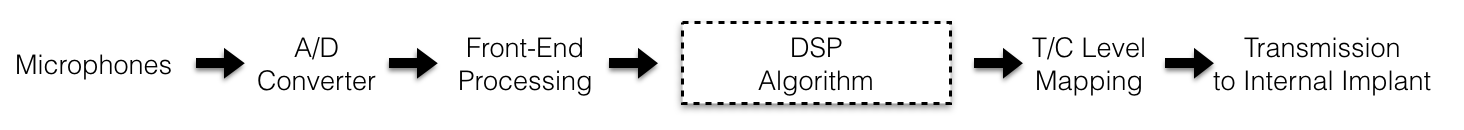
\includegraphics[width=1.0\textwidth]{CI_Signal_FlowTEMP}   
    \caption{Signal Flow in CI}
\end{figure}

\subsection{ACE}

The simplest of the considered strategies is the Advanced Combination Encoder (ACE).  ACE has become a clinical standard for CI processing and is used in a vast number of users.  In essence, hilbert envelopes are extracted from the signal using 

\begin{figure}[!ht]
  \centering
    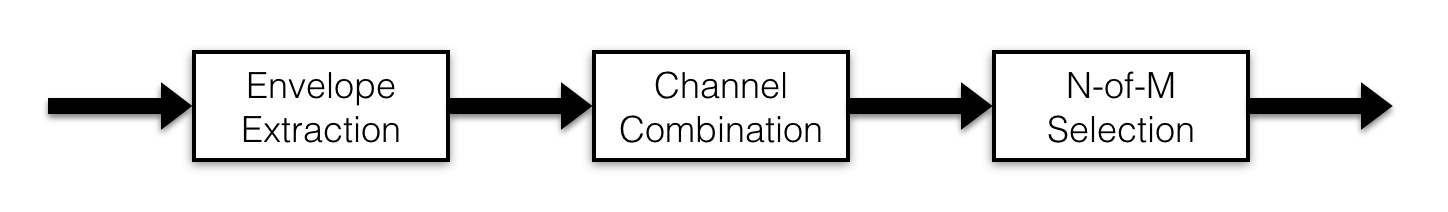
\includegraphics[width=0.5\textwidth]{ACE_flow_diagramTEMP}   
    \caption{ACE Flow Diagram}
\end{figure}

While ACE does a sufficient job for most CI users in speech recognition tasks, a large gap remains between NH and CI in pitch discrimination.  ACE uses place cues as the primary source of encoding a sound's characteristics.  To this day it is still unclear as to what implications this has.  This is due to a combination of factors including the subjective nature of pitch and absence of a ground truth baseline in many CI users.  For example, high-pass filtering a sound may cause it to sound brighter.  In contrast low-pass filtering would cause a warm quality.  As stimulus change electrodes a CI user could claim to experience changes in the high-low quality of pitch when really they are experiencing changes in the bright-warm quality of spectral distribution, or more likely an ambiguous combination of both.

There is general consensus that place cues are not sufficient for encoding pitch.  Alternatively, temporal cues encoded as time-domain carrier modulations have shown to be promising.

ACE currently uses modulations due to harmonic artifacts and low-order FFT.  This is horrible!  Let me explain why...it has nothing to do with the harmonic of interest and everything to do with the one harmonic below and one harmonic above the harmonic of interest.  Because this demodulation is done incoherently the modulation rates are not exactly at $F_0$ and even worse, they aren't aligned with one another (what are the implications of this?).  Furthermore, the cutoff is fixed and decided by parameters of the FFT and sampling rate which have nothing to do with the signal itself.  (Could this also theoretically be a problem for F0mod?  Case: $F_0$ is very low and the harmonic lands right between two bins.  A small modulation could come about, ~probably not~)

\subsection{F0mod}

To get at the problem of pitch discrimination, (Laneau et al 2006) developed a new research strategy, F0mod.  F0mod provides the same processing as ACE with one important change, explicit carrier modulation.  It achieves this by adding a pitch estimator into the processing.

Once a fundamental frequency ($F_0$) is acquired, all output envelopes are modulated by a raised sinusoid at a rate of $F_0$.  This raised sinusoid is constant modulation depth, (full dynamic range), and same across channels, (phase aligned).  *maybe show a figure?  The details of modulator type are discussed later in section ?.?.  The important point here is that modulations are applied at a rate of $F_0$.

An important detail to note is that of low-order-FFT induced modulations mentioned for ACE.  Laneau explicitly describes two different methods as ACE128 and ACE512 corresponding to different FFT orders.  F0mod uses ACE512 which keeps FFT bin modulations below roughly 60Hz in contrast to ACE128's 240Hz.  This sharper cutoff keeps envelope modulations out of the carrier frequency range, isolating this component and leaving the role of carrier modulation to the explicit modulator at $F_0$.

This segregation allows for easier relation to the modulation model of sounds.  Furthermore, F0mod is not prone to the modulation artifacts present in ACE128 and discussed in section 2.?.?

\begin{figure}[!ht]
  \centering
    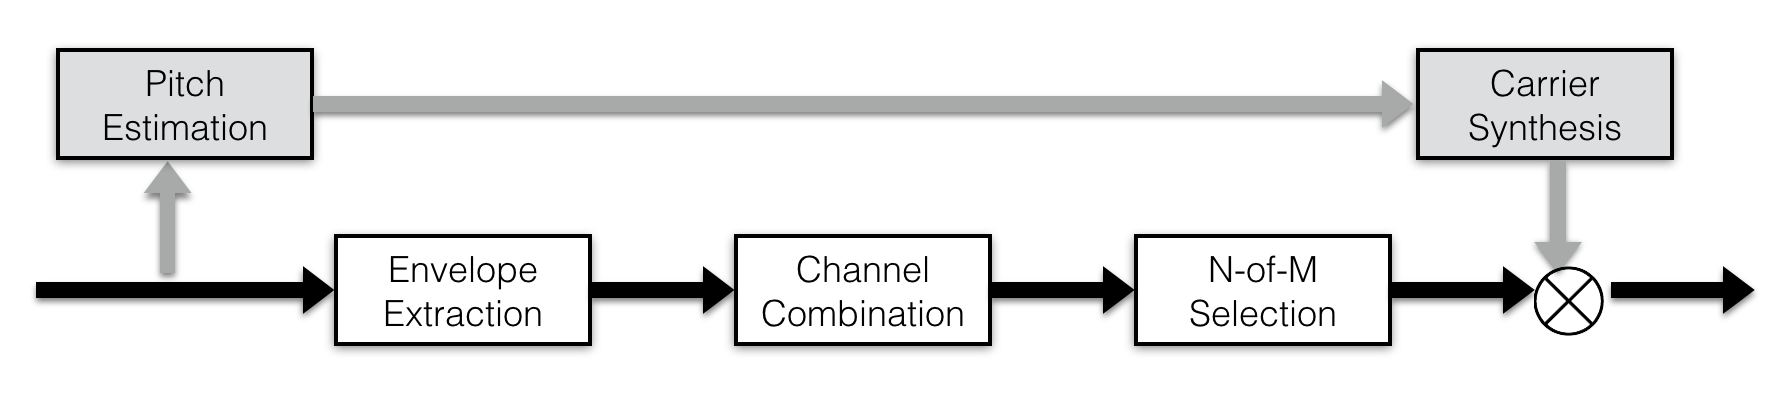
\includegraphics[width=0.5\textwidth]{F0mod_flow_diagramTEMP}   
    \caption{F0mod Flow Diagram}
\end{figure}

F0mod has shown promising results in acute tests for pitch discrimination.  It has also inspired other processing strategies such as eTone, which uses a more sophisticated harmonic sieve pitch estimator as well as soft decisions to overcome the problem of encoding both harmonic and inharmonic sounds as well as those that fall somewhere in between.

\subsection{HSSE}

Looking for a novel approach to improved pitch perception and more broadly music perception, (Li, Atlas, Nie) came up with HSSE.  HSSE uses coherent demodulation to extract harmonic envelopes.  These envelopes are then combined with carrier modulators, just as in F0mod.  These combined carrier-envelope modulators are then assigned to channels based on the harmonic index and $F_0$.

\begin{figure}[!ht]
  \centering
    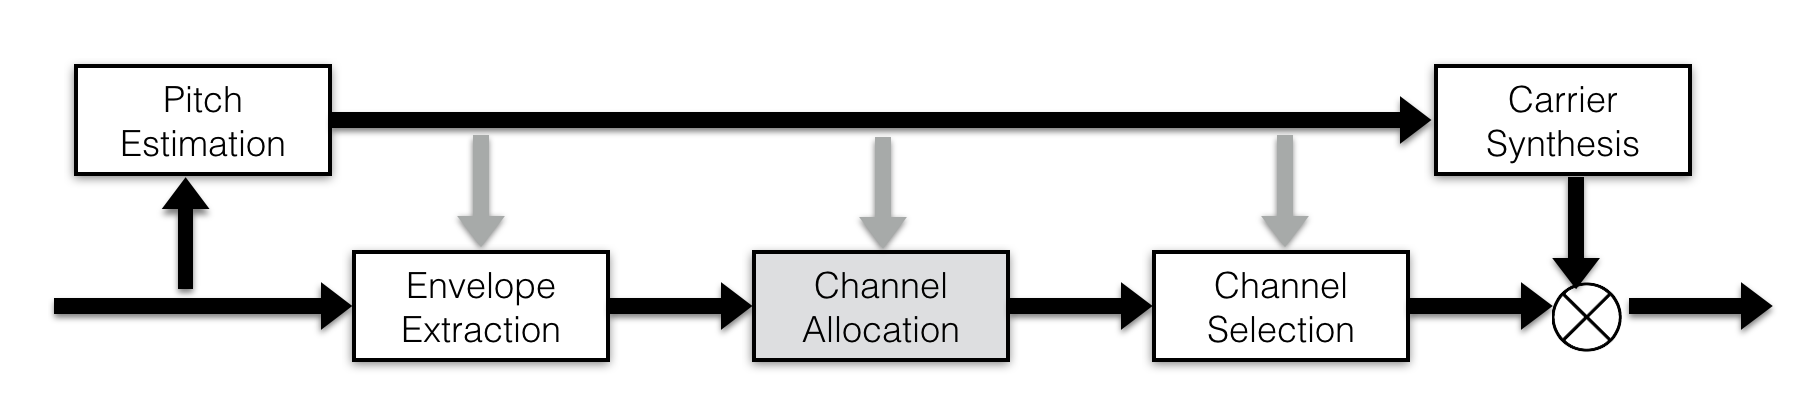
\includegraphics[width=0.5\textwidth]{HSSE_flow_diagramTEMP}   
    \caption{HSSE Flow Diagram}
\end{figure}

Sparing details which we will soon investigate deeper, the differences between F0mod and HSSE can be summarized in two simple points:

1) Envelope extraction is done coherently using $F_0$ from the pitch estimator.

2) Selection and Mapping are now on a different type of envelope and new considerations must be taken into account.


I will argue that all differences can actually be isolated to the envelope extraction stage, however, an important background topic must first be discussed.


\subsection{Selection \& Mapping}

ACE is Cochlear Ltd's instance of the auditory community's generalized category of $N$-of-$M$ strategies.  $M$ is the number of electrodes (or channels) that may be activated and $N$ is the number of electrodes active during any one stimulation frame, $N \leq M$.  In these strategies an incoming audio stream is fed into a filter bank which then computes $M$ modulator envelopes.  In each processing frame, $N$ maxima are chosen from the envelopes and are then mapped to their associated electrodes.  $M \leq$ the number of electrodes on the device, so envelope to electrode is a simple 1-1 map.

It is important to note that this is the same case for F0mod.  The carrier modulation is the same on each envelope and thus does not affect the selection process.

\begin{figure}[!ht]
  \centering
    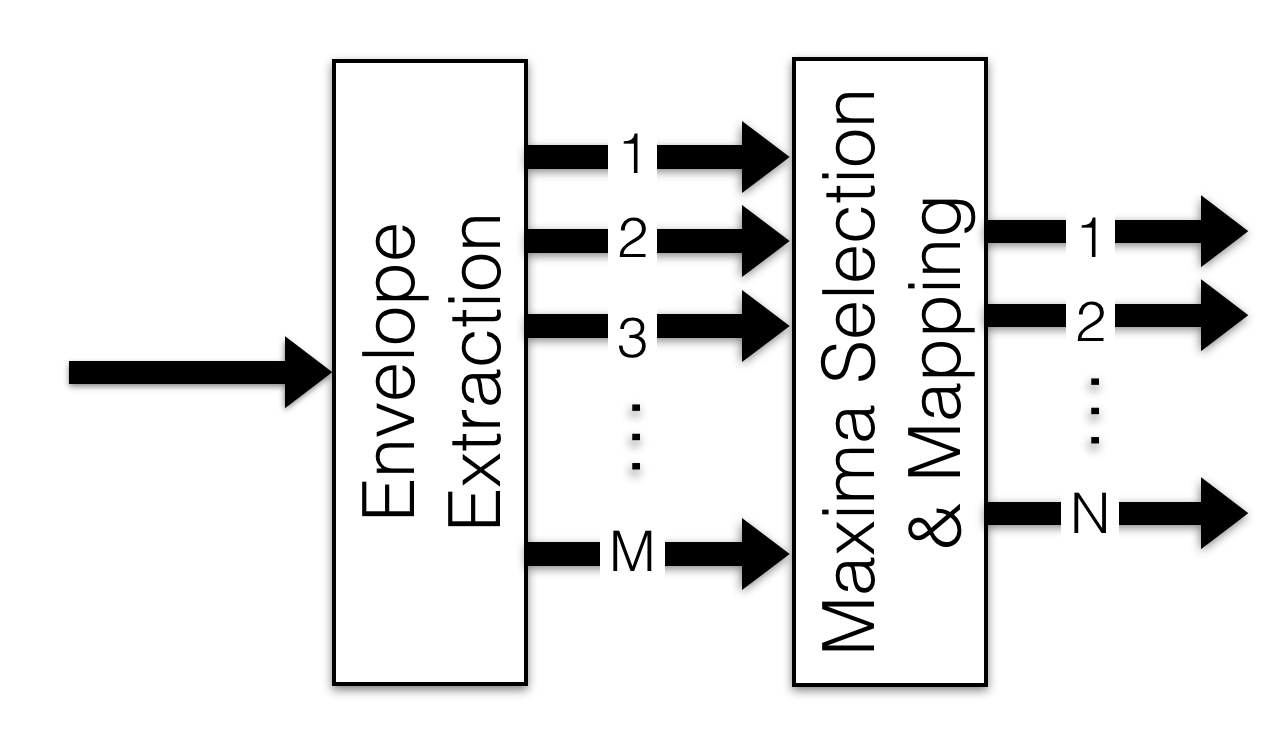
\includegraphics[width=0.5\textwidth]{ACE_selectionTEMP}   
    \caption{N-of-M Maxima Selection}
\end{figure}

On the other hand, HSSE outputs $H$ harmonic envelopes, (one modulator envelope per harmonic).  In this case, it is possible to have $H>N$ but ultimately it must be slimmed down to $N$ envelopes per frame.  Various ideas have been proposed including $N$-largest and lowest-$N$.  Fixed Greenwood bands are determined offline, corresponding each electrode with a bandwidth.  The $N$ envelopes are then mapped to electrodes by finding the greenwood bands each harmonic falls within.

\begin{figure}[!ht]
  \centering
    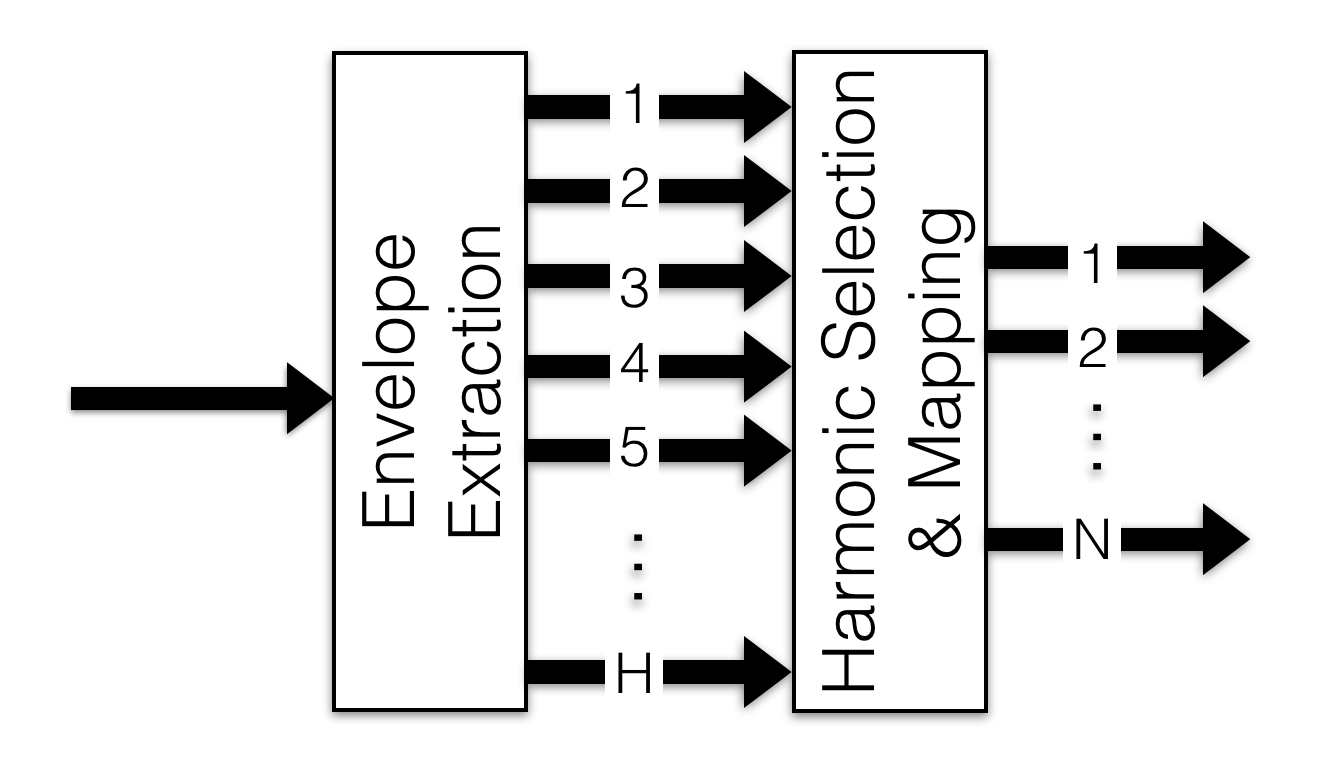
\includegraphics[width=0.5\textwidth]{HSSE_selection_oldTEMP}   
    \caption{N-of-H Harmonic Selection}
\end{figure}



In HSSE it still holds true that $N \leq M$.  While it may seem unnecessary, we could add intermediate steps where first $N$ of $M$ envelopes are set based on some harmonic selection process, then the remaining $M-N$ envelopes are set to zero.  The second stage would be $N$-of-$M$ maxima selection and mapping exactly as is done in ACE.

The added $M-N$ zero expansion give us a new way of interpreting HSSE where an identity-like operation is performed by a selection/mapping stage exactly the same as in ACE.

\begin{figure}[!ht]
  \centering
    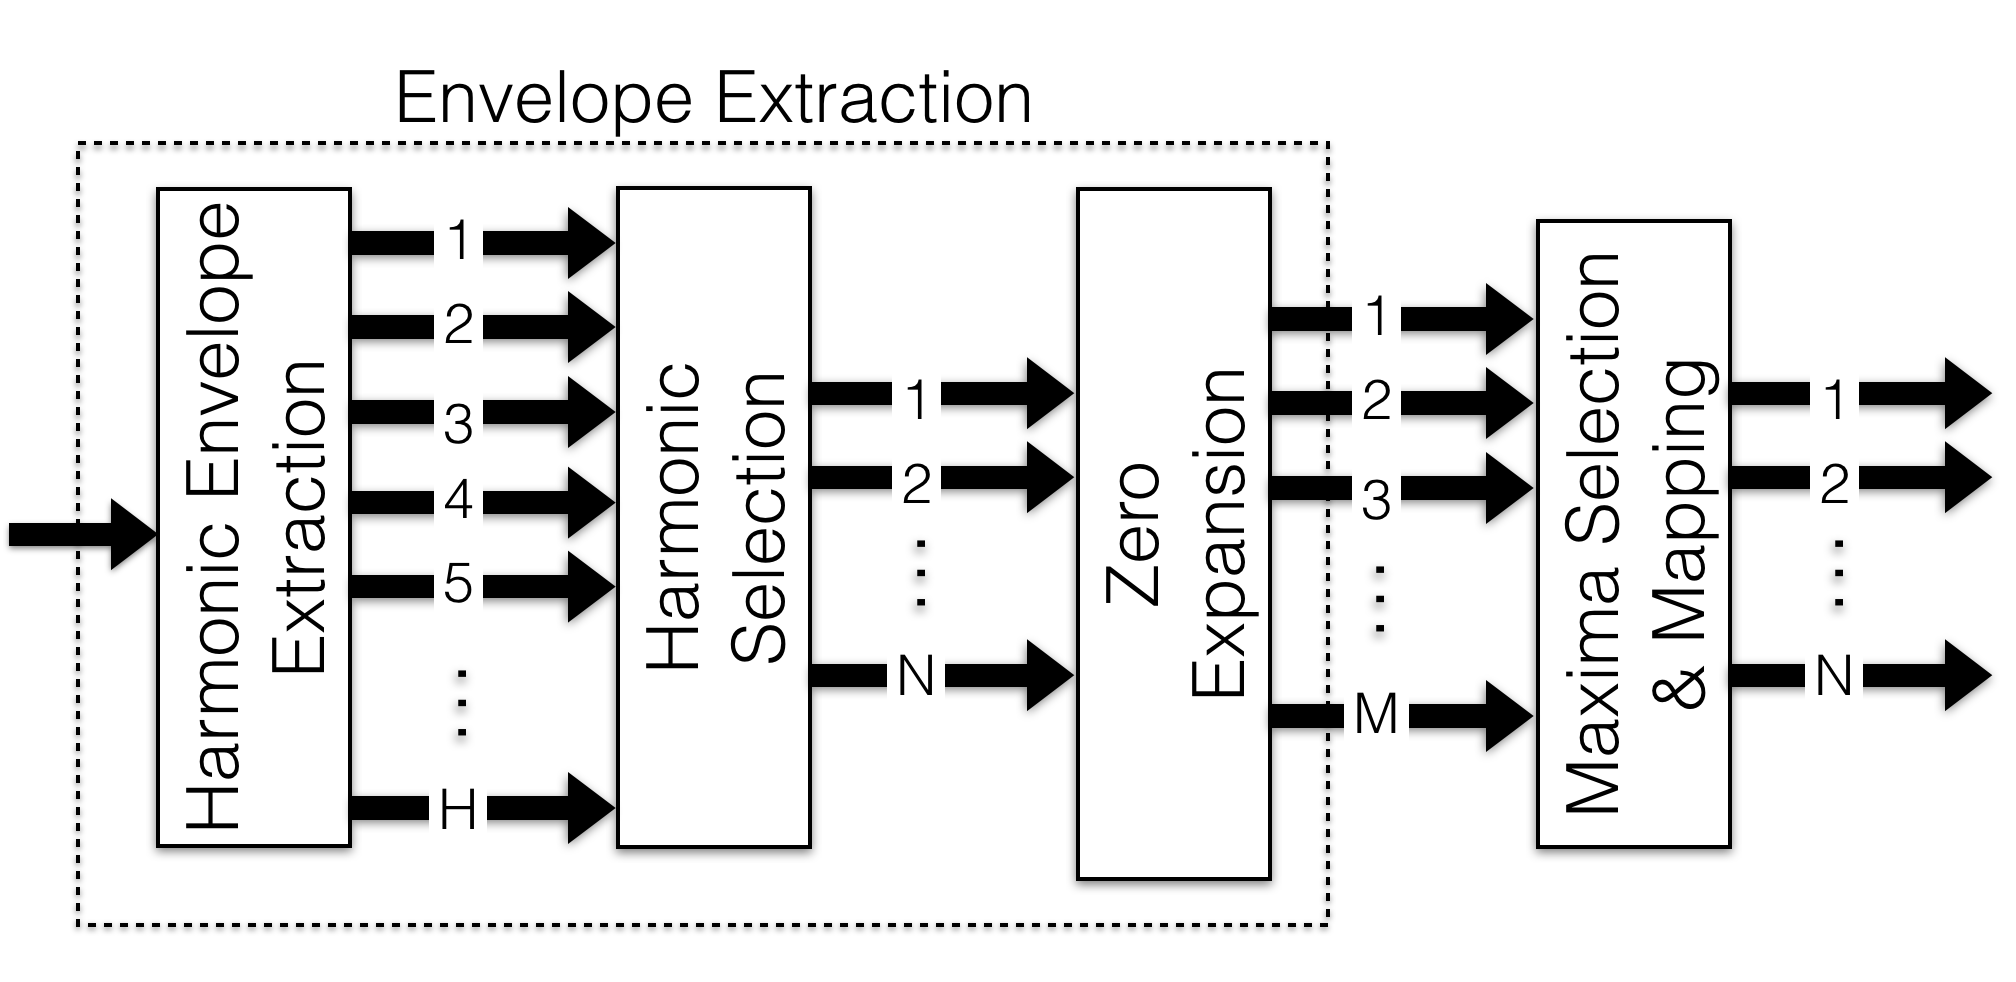
\includegraphics[width=0.8\textwidth]{HSSE_selection_newTEMP}   
    \caption{Reinterpreted N-of-H as N-of-M}
\end{figure}

Keeping this in consideration, we can append harmonic selection to the envelope extraction block in HSSE with the benefit to analysis that all differences between F0mod and HSSE are contained in this envelope extraction stage.


\subsection{Other Strategies}

any hybrid considerations?  maybe hint at hsse ace hybrid

talk about unmentioned methods (AB, MedEl)

\subsection{Summary}

To summarize, the considered strategies can be described by three general processing blocks, Pitch Estimation, Envelope Extraction and Selection \& Mapping.

1) Pitch Estimation

Fundamental Frequency Modulation is a key prospect in temporal encoding, shared by F0mod and HSSE, but not ACE.  There are various ways to estimate pitch with trade-offs for each.  We are going to assume the pitch estimator is the same when analyzing F0mod and HSSE.

2) Envelope Extraction

This has not been talked about in detail intentionally.  The goal of this section was preparation and justification of a deeper analysis of envelope extraction methods.

3) Selection and Mapping

By appending harmonic selection to the envelope extraction block analysis becomes simpler in that all strategies are the same within the selection and mapping block.


\section{Envelope Extraction Methods}

This is about Coherent vs Incoherent Envelopes and the details of each Incoherent method

how much detail are we going into?  Compare CIS, ACE, Hilbert.  Compare ACE128 to ACE512...

where do the matlab figs fall into play here?? (probably way later after math, etc)

Let's do more detailed figures highlighting the differences between F0mod/ACE and HSSE envelope techniques!

Fig: FFT -> Sum into Channels

Fig: Coherent Demod, maybe we need to talk about types of coherent envelopes first?

up until now we haven't needed to be explicit in what envelopes we are talking about, we now need to define these various terms:

incoherent vs coherent

harmonic vs hilbert (FFT bin)


\subsection{Why We Can't Take Real}

I think that this stems from the complex filter.  If our $F_0$ estimate is off by just the slightest bit, then the energy of the signal shifts into the imaginary component.  As a result the energy seems to be lost when taking the real.

furthermore, phase alignment has proven to be imprtant in both HSSE and F0mod

reduces the posibilites to just rectification, instead of various forms of modulation possible in CIs

phase alignment has been found to be important


\subsection{Coherent is the Same (mathematically) as Hilbert, as ACE, as CIS except...}

...for the downshift frequency

\subsection{Bin Alignment}

The human ear has much better resolution than the cochlear implant sound processor when decomposing a signal into frequency bands.  The artifacts of this can be clearly demonstrated by example.  In case1, the energy of the signal falls directly on the center frequency of an FFT bin.  In case2 the signal falls in between two bins.  In this case, neither bin represents the true energy of the signal.

\section{Alternative Coherent Envelope Calculation using FFT bins}

This could all be achieved by zero padding

Math math math!

Incredibly frustrating...but do we even need this?  What about just choosing the nearest FFT bin.

Another consideration: 

\section{Critical Bands}

\subsection{HSSE vs ACE vs Human Ear}

In this subsection I will discuss the general differences in critical bandwidth:

1) how HSSE is too fine of a resolution
note: HSSE originaly had BW = F0/2, however hard to implement and still not like ear

2) how ACE is overall a poorer resolution

What about doing a hybrid?  This would further justify alternative HSUM in it's improved efficiency!  If summing together anyway, does it matter if harmonic envelopes are used or incoherent envelopes are used?

How about specifying the bandwidth at each electrode as apposed to the frequency boundaries

Bro, you need to look into Xing's method with multiple harmonics modulated at multiples of F0...
%curK in HSSE_all_harmonics_halfF0_8_dynamic_channel_Xing.m


\subsection{Resolution Simulated by Adaptive Envelopes}

The human ear has orders of magnitude more filters than ACE, (roughly 1500/22 I think).

HSSE could simulate this higher resolution by choosing different filter center frequencies based on the input signal

\subsection{Channel Selection Analysis}

ACE is like HSSE but for fixed FoI's.  We extract an envelope at the FoI and then transmit it to the associated electrode.

1) this goes back to what are the implications of ACE512 vs ACE128 vs coherent-envelope if we are summing anyway

2) can HSSE be reanalyzed in these terms to better justify wide-bandwidth filters for high frequencies?

Could channel selection concepts in HSSE be important?  Reflect on this in hindsight to recent discoveries.  By this I mean using memory to not switch channels excessively and other decisions that were brought into account.

\section{Other Important Components}

Most everything so far has assumed the signal has an $F_0$, what if it doesn't?  What if it is well outside the boundaries of $F_0$?  What about polyphonic music?  What about SNRs below what is needed for accurate $F_0$ estimation.  What other flaws do these strategies have?  Mention eTone and other possible solutions, or why we justify not considering these problems.
 
% ========== Chapter 3

\chapter{New Attempt: HSSE vs F0mod}

\section{The Components}

1) Envelope Extraction

2) Channel Combination

3) Channel Selection

\section{Envelope Extraction}

\subsection{Magnitude}

I have looked into a few different ways to get magnitude envelopes.  As it turns out...they're all pretty much the same.

\subsection{Real}

Not sure where this is going to lead me

I think that this stems from the complex filter.  If our $F_0$ estimate is off by just the slightest bit, then the energy of the signal shifts into the imaginary component.  As a result the energy seems to be lost when taking the real.

furthermore, phase alignment has proven to be imprtant in both HSSE and F0mod

reduces the posibilites to just rectification, instead of various forms of modulation possible in CIs

phase alignment has been found to be important.  Can we do real version without phase misalignment problem?

\section{Channel Combination}

does remanian/geodesic distance have anything to do with sum of squares?  I think it's just euclidean...

What does bin summing mean?  How does it compare to sinc interpolation?

What happens when bins are summed?  Does gain change or do the bins just become averaged?  In that sense, how important is the gain stage?  What are those gains?

What if we did F0mod with same channel selections as HSSE?  What would happen?

\section{Analysis Directions}

0 - F0mod
1 - HSSE
envelope extraction | channel combination | channel selection

EE | CC | CS

0 | 0 | 0 

0 | 0 | 1

...


% ========== Chapter 4
 
\chapter{Less Theoretical Stuff}

About this chappy

\section{Engineering Decisions for Real-time}

1) 8 harmonics
this assumes we are dealing with musical instruments, speech is going to have characteristics well above the 8th harmonic.  A hope is that with inharmonic signals the estimate will automatically bounce to max($F_0$ estimate) which will thus hit the highest frequencies.  This also goes back to the hybrid idea


2) $F_0$ estimation downsampling details, ooOOooo, so impressive!

\section{$F_0$ tilt, exageration}

mention the point that this was already done in Xing's paper, albeit $F_0/2$ without affine shift is more more likely to hit boundaries 

\section{Modulation Types}


%
% ==========   Bibliography
%
\nocite{*}   % include everything in the uwthesis.bib file
\bibliographystyle{plain}
\bibliography{uwthesis}
%
% ==========   Appendices
%
\appendix
\raggedbottom\sloppy
 
% ========== Appendix A
 
\chapter{Where to find the files}
 
The uwthesis class file, {\tt uwthesis.cls}, contains the parameter settings,
macro definitions, and other \TeX nical commands which
allow \LaTeX\ to format a thesis.  
The source to
the document you are reading, {\tt uwthesis.tex},
contains many formatting examples
which you may find useful.
The bibliography database, {\tt uwthesis.bib}, contains instructions
to BibTeX to create and format the bibliography.
You can find the latest of these files on:

\begin{itemize}
\item My page.
\begin{description}
\item[] \verb%http://staff.washington.edu/fox/tex/uwthesis.html%
\end{description}

\item CTAN
\begin{description}
\item[]  \verb%http://tug.ctan.org/tex-archive/macros/latex/contrib/uwthesis/%
\item[]  (not always as up-to-date as my site)
\end{description}

\end{itemize}

\vita{Jim Fox is a Software Engineer with UW Information Technology at the University of Washington.
His duties do not include maintaining this package.  That is rather
an avocation which he enjoys as time and circumstance allow.

He welcomes your comments to {\tt fox@uw.edu}.
}


\end{document}
